\documentclass[aspectratio=43,9pt]{beamer}
\let\Tiny=\tiny
%
\usepackage{tikz}
\usepackage{enumerate}
%
\usetheme{Boadilla}
%
%
\let\Tiny=\tiny%			% to avoid warnings about font size
%\usepackage{lmodern}%		% alternative method to avoid these warnings
%
\catcode`~=11 % make LaTeX treat tilde (~) like a normal character
\newcommand{\urltilde}{\hbox{~}}
\catcode`~=13 % revert back to treating tilde (~) as an active character
%
% misc commands
\newcommand{\bm}[1]{\mathbf{#1}}
\newcommand{\bs}[1]{\boldsymbol{#1}}
\newenvironment{myitemize}[1]{\vspace{#1}\begin{itemize}\setlength\itemsep{#1}}{\end{itemize}}
%
% pgf markers
\usepgflibrary{plotmarks}
%
\setbeamertemplate{footline}
{
  \leavevmode%
  \hbox{%
  \begin{beamercolorbox}[wd=.8\paperwidth,ht=2.25ex,dp=1ex,left]{author in head/foot}%
    \usebeamerfont{author in head/foot}\hspace*{4em}\inserttitle
  \end{beamercolorbox}%
  \begin{beamercolorbox}[wd=.2\paperwidth,ht=2.25ex,dp=1ex,right]{author in head/foot}%
    \usebeamerfont{author in head/foot}\insertframenumber{} / \inserttotalframenumber\hspace*{1ex}
  \end{beamercolorbox}}%
  \vskip0pt%
}
%
\setbeamertemplate{navigation symbols}{}
%
\setbeamertemplate{frametitle}
{%
	\begin{minipage}{.9\paperwidth}
		\vspace*{1ex}%
		\flushright%
		%\bfseries
		\LARGE%
		\insertframetitle%
	\end{minipage}%
}
%
\setbeamertemplate{title page}{
	\begin{center}
		\vspace*{2ex}
		\usebeamercolor[fg]{frametitle}{%
			\Large%
			Numerical Techniques 2025--2026\\[2ex]
			%
			\LARGE%
			\inserttitle
		}\\[6ex]
		\usebeamercolor[fg]{normal text}{%
			Daan Degrauwe\\[1ex]
			\texttt{daan.degrauwe@meteo.be}\\[4ex]
			Postgraduate Studies in Weather and Climate Modeling\\[1ex]
			Ghent University
		}
	\end{center}
}
%
\newcommand{\ft}[2]{{\textstyle\frac{#1}{#2}}}
%
% increase space around equations
\makeatletter
\g@addto@macro\normalsize{%
	\setlength{\abovedisplayskip}{3ex}%
	\setlength{\belowdisplayskip}{3ex}%
	\setlength{\abovedisplayshortskip}{3ex}%
	\setlength{\belowdisplayshortskip}{3ex}%
}%
\makeatother
%

%
\title{Practicum 1: Linux and Fortran basics}
%
\graphicspath{{figures/}}
%
\begin{document}
%
%%%%%%%%%%%%%%%%%%%%%%%%%%%%%%%%%%%%%%%%%%%%%%%%%%%%%%%%%%%%%%%%%%%%%%%%%%%%%%%%%%%%%%%%%%%%%%%%%%%%
%
\begin{frame}[plain]
	\titlepage
\end{frame}
%
%%%%%%%%%%%%%%%%%%%%%%%%%%%%%%%%%%%%%%%%%%%%%%%%%%%%%%%%%%%%%%%%%%%%%%%%%%%%%%%%%%%%%%%%%%%%%%%%%%%%
%
\begin{frame}
	%
	\frametitle{The problem at hand: the oscillation equation}
	%
	\begin{itemize}
		\item The oscillation is a differential equation given by:
			%
			\begin{equation*}
				\frac{\partial \psi}{\partial t} = i \kappa \psi
			\end{equation*}
			%
		\item The exact solution is a harmonic function with frequency $\kappa$:
			%
			\begin{equation*}
				\psi(t)=e^{i\kappa t}\psi(t_0) = \left(\cos(\kappa t)+i\sin(\kappa t)\right)\psi(t_0)
			\end{equation*}
			%
		\item A simple numerical scheme is the \emph{forward scheme}:
			\begin{equation*}
				\frac{\phi^{t+\Delta t}-\phi^t}{\Delta t}=i\kappa \phi^t
			\end{equation*}
			or
			\begin{equation*}
				\phi^{t+\Delta t}=(1+i\kappa\Delta t) \phi^t
			\end{equation*}			
	\end{itemize}
\end{frame}
%
%%%%%%%%%%%%%%%%%%%%%%%%%%%%%%%%%%%%%%%%%%%%%%%%%%%%%%%%%%%%%%%%%%%%%%%%%%%%%%%%%%%%%%%%%%%%%%%%%%%%
%
\begin{frame}
	%
	\frametitle{Infrastructure: 3 machines}
	%
	\begin{tikzpicture}[>=latex]
		\draw (0,3) node[above]{\bfseries Student};
		\draw (0,2) node(usr1){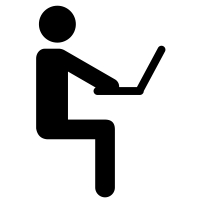
\includegraphics[width=15mm]{laptop_user}};
		\draw (0,0) node(usr2){
\includegraphics[width=15mm]{smartphone_user}};
		\draw (-1.5,-1) node[below right]{\parbox{50mm}{%
			laptop, PC,\\ smartphone, tablet:
			\begin{itemize}
				\item user input
			\end{itemize}
		}};
		\draw (4,3) node[above]{\parbox[t][0pt][t]{40mm}{\centering {\bfseries Athena}\\(https://athena.ugent.be)}};
		\draw (4,1) node(ath){
\includegraphics[width=15mm]{windows_icon}};
		\draw (2.5,-1) node[below right]{\parbox{50mm}{%
			 Windows machine:
			\begin{itemize}
				\item Linux login (PuTTY)
				\item File editing (Notepad++)
				\item Postprocessing (RStudio)
			\end{itemize}
		}};
		\draw (8,3) node[above]{\bfseries helios};
		\draw (8,1) node(hel){
\includegraphics[width=15mm]{linux_icon}};
		\draw (7,-1) node[below right]{\parbox{50mm}{%
			Linux machine:
			\begin{itemize}
				\item compilation (gfortran)
				\item calculations (Fortran)
			\end{itemize}
		}};
		\draw [->,line width=2pt,color=blue!60] (usr1) -- (ath);
		\draw [->,line width=2pt,color=blue!60] (usr2) -- (ath);
		\draw [->,line width=2pt,color=blue!60] (ath) -- (hel);
	\end{tikzpicture}\hspace*{-.5\textwidth}
\end{frame}
%
%%%%%%%%%%%%%%%%%%%%%%%%%%%%%%%%%%%%%%%%%%%%%%%%%%%%%%%%%%%%%%%%%%%%%%
%
\begin{frame}
	%
	\frametitle{Logging in}
	%
	\begin{enumerate}
		\item Create helios account on \texttt{https://helpdesk.ugent.be/account/en/helios.php}\vspace*{2ex}
		\item Log in on Athena on \texttt{https://athena.ugent.be}\vspace*{2ex}
		\item Open PuTTY on Athena\vspace*{2ex}
		\item Set Host Name to \emph{helios.ugent.be}\vspace*{2ex}
		\item Click ``Open'' button
	\end{enumerate}
	%
\end{frame}
%
%%%%%%%%%%%%%%%%%%%%%%%%%%%%%%%%%%%%%%%%%%%%%%%%%%%%%%%%%%%%%%%%%%%%%%
%
\begin{frame}
	%
	\frametitle{Mounting H-drive}
	%
	Do this every time you login on helios!\vspace*{4ex}
	%
	\begin{enumerate}
		\item on helios, mount the H-drive with
			\par\vspace*{1ex}\hspace*{.05\textwidth}\parbox{.5\textwidth}{\ttfamily
		   \$   newns  -i
			}\vspace*{1ex}\par\vspace*{2ex}
		\item go to the H-drive with
			\par\vspace*{1ex}\hspace*{.05\textwidth}\parbox{.5\textwidth}{\ttfamily
		   \$   cd  /files/\$\string{USER\string}/home/
			}\vspace*{1ex}\par
			(where you can substitute \texttt{\$\string{USER\string}} by your user)
	\end{enumerate}
	%
\end{frame}
%
%%%%%%%%%%%%%%%%%%%%%%%%%%%%%%%%%%%%%%%%%%%%%%%%%%%%%%%%%%%%%%%%%%%%%%
%
\begin{frame}
	%
	\frametitle{Creating and modifying a text file}
	%
	\begin{enumerate}
		\item on helios, create an empty file with
			\par\vspace*{1ex}\hspace*{.05\textwidth}\parbox{.5\textwidth}{\ttfamily
				\$   mkdir  /files/\$\string{USER\string}/home/numtech\\
				\$   cd  /files/\$\string{USER\string}/home/numtech\\
				\$   touch  test.txt
			}\vspace*{1ex}\par\vspace*{2ex}
		\item on Athena, open Notepad++\vspace*{2ex}
		\item inside {Notepad++}, open the file \texttt{H:/numtech/test.txt}, and put some text in it\vspace*{2ex}
		\item \textbf{Important}: set the end-of-line convention under\\ Edit$\rightarrow$EOL Conversion$\rightarrow$Unix/OSX Format\\ Do this always for files you will use in Linux!\vspace*{2ex}
		\item Save the file in Notepad++\vspace*{2ex}
		\item on helios, check the file content with
			\par\vspace*{1ex}\hspace*{.05\textwidth}\parbox{.5\textwidth}{\ttfamily
				\$   cat  test.txt
			}\vspace*{1ex}\par
	\end{enumerate}
	%
\end{frame}
%
%%%%%%%%%%%%%%%%%%%%%%%%%%%%%%%%%%%%%%%%%%%%%%%%%%%%%%%%%%%%%%%%%%%%%%
%
\begin{frame}
	%
	\frametitle{My first Fortran program}
	%
	\begin{enumerate}
		\item create a file \texttt{osceq.F90}:
			\par\vspace*{1ex}\hspace*{.05\textwidth}\parbox{.8\textwidth}{\ttfamily
				\$   mkdir  /files/\$\string{USER\string}/home/numtech/osceq\\
				\$   cd  /files/\$\string{USER\string}/home/numtech/osceq\\
				\$   touch  osceq.F90
			}\vspace*{1ex}\par\vspace*{2ex}
		\item open the file in Notepad++, and put following code in it:
			\par\vspace*{1ex}\hspace*{.05\textwidth}\parbox{.8\textwidth}{\ttfamily\small
				PROGRAM OSCEQ\\[3ex]
				! a program to solve the oscillation equation\\[3ex]
				WRITE (*,*) "Welcome to the Oscillation Equation Solver."\\[3ex]
				END PROGRAM OSCEQ
			}\hspace*{-.5\textwidth}\vspace*{1ex}\par\vspace*{2ex}
		\item compile the program with
			\par\vspace*{1ex}\hspace*{.05\textwidth}\parbox{.5\textwidth}{\ttfamily
				\$   gfortran -o osceq osceq.F90
			}\vspace*{1ex}\par\vspace*{2ex}
		\item run the program with
			\par\vspace*{1ex}\hspace*{.05\textwidth}\parbox{.5\textwidth}{\ttfamily
				\$   ./osceq
			}\vspace*{1ex}\par
	\end{enumerate}
	%
\end{frame}
%
%%%%%%%%%%%%%%%%%%%%%%%%%%%%%%%%%%%%%%%%%%%%%%%%%%%%%%%%%%%%%%%%%%%%%%
%
\begin{frame}
	%
	\frametitle{My first Linux script}
	%
	\begin{enumerate}
		\item create a file \texttt{run.sh}
			\par\vspace*{1ex}\hspace*{.05\textwidth}\parbox{.5\textwidth}{\ttfamily
				\$   touch  run.sh\\
				\$   chmod  +x  run.sh
			}\vspace*{1ex}\par
		\item open the file in Notepad++, and put following code in it:
			\par\vspace*{1ex}\hspace*{.05\textwidth}\parbox{.8\textwidth}{\ttfamily\small
				\# Script to compile and run the oscillation equation program\\[3ex]
				\# remove executable file\\
				rm osceq\\[3ex]
				\# Compile\\
				echo "Compiling"\\
				gfortran -o osceq osceq.F90\\[3ex]
				\# Run\\
				echo "Running"\\
				./osceq
			}\vspace*{1ex}\par
		\item compiling and running are now done together with
			\par\vspace*{1ex}\hspace*{.05\textwidth}\parbox{.5\textwidth}{\ttfamily
				\$   ./run.sh
			}\vspace*{1ex}\par
	\end{enumerate}
	%
\end{frame}
%
%%%%%%%%%%%%%%%%%%%%%%%%%%%%%%%%%%%%%%%%%%%%%%%%%%%%%%%%%%%%%%%%%%%%%%
%
\begin{frame}
	%
	\frametitle{Fortran variables}
	%
	\begin{enumerate}
		\item It's good practice to take a copy before moving to the next assignment:
			\par\vspace*{1ex}\hspace*{.05\textwidth}\parbox{.5\textwidth}{\ttfamily
				\$   cp -r ../osceq/ ../osceq\_v1
			}\vspace*{1ex}\par			
		\item \emph{Declare} variables with \texttt{REAL}, \texttt{INTEGER}, \texttt{CHARACTER}, \ldots:
			\par\vspace*{1ex}\hspace*{.05\textwidth}\parbox{.8\textwidth}{\ttfamily\small
				\textcolor{green!80!black}{REAL}    :: KAPPA
			}\vspace*{1ex}\par
		\item \emph{Initialize} variables:
			\par\vspace*{1ex}\hspace*{.05\textwidth}\parbox{.8\textwidth}{\ttfamily\small
				KAPPA \textcolor{green!80!black}{=} 0.5
			}\vspace*{1ex}\par
		\item \emph{Use} variables in expressions:
			\par\vspace*{1ex}\hspace*{.05\textwidth}\parbox{.8\textwidth}{\ttfamily\small
				WRITE (*,*) 'CFL = ',\textcolor{green!80!black}{KAPPA}*DT
			}\vspace*{1ex}\par			
	\end{enumerate}
	%
\end{frame}
%
%%%%%%%%%%%%%%%%%%%%%%%%%%%%%%%%%%%%%%%%%%%%%%%%%%%%%%%%%%%%%%%%%%%%%%
%
\begin{frame}
	%
	\frametitle{Fortran loops and conditions}
	%
	\begin{enumerate}	
		\item Repetitive tasks (like a time integration) are implemented with Fortran loops:
			\par\vspace*{1ex}\hspace*{.05\textwidth}\parbox{.8\textwidth}{\ttfamily\small
				\textcolor{green!80!black}{DO} IT=1,NT\\
				\hspace*{2em}!...\\
				\textcolor{green!80!black}{ENDDO}
			}\vspace*{1ex}\par
		\item Conditional branching is achieved with \texttt{IF}:
			\par\vspace*{1ex}\hspace*{.05\textwidth}\parbox{.8\textwidth}{\ttfamily\small
				\textcolor{green!80!black}{IF} ( ABS(PHI) > 10. ) \textcolor{green!80!black}{THEN}\\
				\hspace*{2em}!...\\
				\textcolor{green!80!black}{ENDIF}
			}\vspace*{1ex}\par
	\end{enumerate}
	%
\end{frame}
%
%%%%%%%%%%%%%%%%%%%%%%%%%%%%%%%%%%%%%%%%%%%%%%%%%%%%%%%%%%%%%%%%%%%%%%
%
\begin{frame}
	%
	\frametitle{Fortran arrays}
	%
	Arrays contain a collection of numbers.
	%
	\begin{enumerate}	
		\item Declaration with \texttt{ALLOCATABLE} attribute and dimension indication:
			\par\vspace*{1ex}\hspace*{.05\textwidth}\parbox{.8\textwidth}{\ttfamily\small
				COMPLEX, \textcolor{green!80!black}{ALLOCATABLE} :: PSI(:)
			}\vspace*{1ex}\par
		\item Allocation (memory reservation) with \texttt{ALLOCATE}:
			\par\vspace*{1ex}\hspace*{.05\textwidth}\parbox{.8\textwidth}{\ttfamily\small
				\textcolor{green!80!black}{ALLOCATE}(PSI(0:NT))
			}\vspace*{1ex}\par
		\item Reference to an element with \texttt{()}:
			\par\vspace*{1ex}\hspace*{.05\textwidth}\parbox{.8\textwidth}{\ttfamily\small
				PSI\textcolor{green!80!black}{(IT)} = EXP(II*KAPPA*IT*DT)
			}\vspace*{1ex}\par
		\item Free memory with \texttt{DEALLOCATE}:
			\par\vspace*{1ex}\hspace*{.05\textwidth}\parbox{.8\textwidth}{\ttfamily\small
				\textcolor{green!80!black}{DEALLOCATE}(PSI)
			}\vspace*{1ex}\par
		\item Be careful not to exceed the bounds of an array! Compile with bound checking for security:
			\par\vspace*{1ex}\hspace*{.05\textwidth}\parbox{.8\textwidth}{\ttfamily
				\$   gfortran -fbounds-check -o osceq osceq.F90
			}\vspace*{1ex}\par					
	\end{enumerate}
	%
\end{frame}
%
%%%%%%%%%%%%%%%%%%%%%%%%%%%%%%%%%%%%%%%%%%%%%%%%%%%%%%%%%%%%%%%%%%%%%%
%
\begin{frame}
	%
	\frametitle{Fortran subroutines}
	%
	Use subroutines to organize your code.\vspace*{2ex}
	%
	\begin{enumerate}	
		\item Separate subroutines best go in separate files.
		\item Arguments are declared with the \texttt{INTENT} attribute:
			\par\vspace*{1ex}\hspace*{.05\textwidth}\parbox{.8\textwidth}{\ttfamily\small
				\textcolor{green!80!black}{SUBROUTINE} WRITE\_RESULT(PSI,PHI)\\[3ex]
				REAL, \textcolor{green!80!black}{INTENT(IN)} :: PSI(:)\\
				REAL, \textcolor{green!80!black}{INTENT(IN)} :: PHI(:)\\[3ex]
				!...\\[3ex]
				\textcolor{green!80!black}{END SUBROUTINE} WRITE\_RESULT
			}\vspace*{1ex}\par
		\item Routines are called with \texttt{CALL}:
			\par\vspace*{1ex}\hspace*{.05\textwidth}\parbox{.8\textwidth}{\ttfamily\small
				\textcolor{green!80!black}{CALL} WRITE\_RESULTS(PSI,PHI)
			}\vspace*{1ex}\par
	\end{enumerate}
	%
\end{frame}
%
%%%%%%%%%%%%%%%%%%%%%%%%%%%%%%%%%%%%%%%%%%%%%%%%%%%%%%%%%%%%%%%%%%%%%%
%
\begin{frame}
	%
	\frametitle{Fortran modules}
	%
	Modules are useful to store global data (i.e. data not specific to a single subroutine).
	%
	\begin{enumerate}	
		\item Modules just contain the declarations:
			\par\vspace*{1ex}\hspace*{.05\textwidth}\parbox{.8\textwidth}{\ttfamily\small
				\textcolor{green!80!black}{MODULE} CONSTANTS\\[3ex]
				\parbox{10em}{INTEGER} :: NT\hspace*{3em} ! number of timesteps	\\
				\parbox{10em}{REAL   } :: DT\hspace*{3em} ! timestep size	\\[3ex]
				\textcolor{green!80!black}{END MODULE} CONSTANTS
			}\vspace*{1ex}\par
		\item Subroutines can access the variables from a module with the \texttt{USE} statement:
			\par\vspace*{1ex}\hspace*{.05\textwidth}\parbox{.8\textwidth}{\ttfamily\small
				\textcolor{green!80!black}{USE} CONSTANTS
			}\vspace*{1ex}\par
		\item During compilation, make sure to put files containing modules first:
			\par\vspace*{1ex}\hspace*{.05\textwidth}\parbox{.85\textwidth}{\ttfamily
				\$   gfortran \textcolor{green!80!black}{constants.F90} setup\_constants.F90 timeloop.F90 \string\ \\
				\hspace*{4em}write\_result.F90 osceq.F90 -o osceq
			}\vspace*{1ex}\par		
	\end{enumerate}
	%
\end{frame}
%
%%%%%%%%%%%%%%%%%%%%%%%%%%%%%%%%%%%%%%%%%%%%%%%%%%%%%%%%%%%%%%%%%%%%%%
%
\begin{frame}
	%
	\frametitle{Postprocessing in RStudio}
	%
	\begin{enumerate}	
		\item On Athena, open RStudio\vspace*{2ex}
		\item Load the results file \texttt{output.dat} with
			\par\vspace*{1ex}\hspace*{.05\textwidth}\parbox{.8\textwidth}{\ttfamily
				y=read.table('output.dat',header=TRUE)
			}\vspace*{1ex}\par\vspace*{2ex}
		\item Plot the exact solution with
			\par\vspace*{1ex}\hspace*{.05\textwidth}\parbox{.8\textwidth}{\ttfamily
				plot(y\$time,y\$exact,ylim=c(-3,3),type='b',pch=1,col=1)
			}\vspace*{1ex}\par\vspace*{2ex}
		\item add the numerical solution to the plot with
			\par\vspace*{1ex}\hspace*{.05\textwidth}\parbox{.8\textwidth}{\ttfamily
				points(y\$time,y\$numerical,type='b',pch=2,col=2)
			}\vspace*{1ex}\par\vspace*{2ex}
		\item put these commands in a file \texttt{show\_results.R}, and run it in RStudio with
			\par\vspace*{1ex}\hspace*{.05\textwidth}\parbox{.8\textwidth}{\ttfamily
				source('show\_results.R')
			}\vspace*{1ex}\par
	\end{enumerate}
	%
\end{frame}
%
%%%%%%%%%%%%%%%%%%%%%%%%%%%%%%%%%%%%%%%%%%%%%%%%%%%%%%%%%%%%%%%%%%%%%%
%
\begin{frame}
	%
	\frametitle{Exercises on time schemes}
	%
	\begin{enumerate}	
		\item Implement the backward and the trapezium schemes. What about their stability and phase error?
			\begin{align*}
				\phi^{n+1}&=\frac{1}{1-i\kappa\Delta t}\phi^n&&\text{(backward)}	\\
				\phi^{n+1}&=\frac{1+0.5i\kappa\Delta t}{1-0.5i\kappa\Delta t}\phi^n&&\text{(trapezium)}
			\end{align*}\vspace*{2ex}
		\item Implement the Matsuno scheme, and check the damping as a function of $\kappa\Delta t$. Is it accelerating or decelerating?
			\begin{align*}
				\tilde\phi&=(1+i\kappa\Delta t)\phi^{n}\\
				\phi^{n+1}&=\phi^n+i\kappa\Delta t\tilde\phi
			\end{align*}
	\end{enumerate}
	%
\end{frame}
%
%%%%%%%%%%%%%%%%%%%%%%%%%%%%%%%%%%%%%%%%%%%%%%%%%%%%%%%%%%%%%%%%%%%%%%
%
\begin{frame}
	%
	\frametitle{Exercises on time schemes}
	%
	\begin{enumerate}\setcounter{enumi}{2}
		\item Implement the Leapfrog scheme.
			\begin{equation*}
				\phi^{n+1}=\phi^{n-1}+2i\kappa\Delta t\phi^{n}
			\end{equation*}
			%
			\par
			Use the forward scheme during the first timestep:
			\begin{equation*}
				\phi^{1}=(1+i\kappa\Delta t)\phi^{0}
			\end{equation*}\vspace*{2ex}
		\item Try to excite the computational mode in the Leapfrog scheme (by sabotaging the first timestep).\vspace*{2ex}
		\item Implement the Robert-Asselin filter to damp the computational mode.
			\begin{align*}
				\phi^{n+1}&=\overline{\phi^{n-1}}+2i\kappa\Delta t\phi^{n}\\
				\overline{\phi^n}&=\phi^n+\gamma\left(\overline{\phi^{n-1}}-2\phi^n+\phi^{n+1}\right)
			\end{align*}
	\end{enumerate}
	%
\end{frame}
%
%%%%%%%%%%%%%%%%%%%%%%%%%%%%%%%%%%%%%%%%%%%%%%%%%%%%%%%%%%%%%%%%%%%%%%
%
\end{document}
%

